\documentclass[11pt]{article}
% Shared preamble for the notes in this repository. pdfLaTeX, TeX Live 2024 or later.
\usepackage[a4paper,margin=2.6cm]{geometry}
\usepackage[T1]{fontenc}
\usepackage{lmodern}
\usepackage{microtype}
\usepackage{amsmath,amssymb,amsthm}
\usepackage{graphicx}
\usepackage{booktabs}
\usepackage{enumitem}
\usepackage[dvipsnames]{xcolor}
\usepackage[hidelinks]{hyperref}
\hypersetup{colorlinks=true,linkcolor=MidnightBlue,citecolor=MidnightBlue,urlcolor=MidnightBlue}
\graphicspath{{../../figures/}}
\setlist{itemsep=2pt,topsep=4pt}

\newtheorem{theorem}{Theorem}
\newtheorem{proposition}[theorem]{Proposition}
\newtheorem{corollary}[theorem]{Corollary}
\newtheorem{conjecture}[theorem]{Conjecture}
\theoremstyle{definition}
\newtheorem{definition}[theorem]{Definition}
% Reusable derivations, numbered note.k; each note sets \notenumber. Indexed in DERIVATIONS.md.
\newcommand{\notenumber}{0}
\newtheorem{derivation}{Derivation}
\renewcommand{\thederivation}{\notenumber.\arabic{derivation}}
\newtheorem{question}{Question}
\theoremstyle{remark}
\newtheorem{remark}[theorem]{Remark}

\newcommand{\Z}{\mathbb{Z}}
\newcommand{\Q}{\mathbb{Q}}
\newcommand{\R}{\mathbb{R}}
\newcommand{\C}{\mathbb{C}}
\newcommand{\HH}{\mathbb{H}}
\newcommand{\SL}{\mathrm{SL}}
\newcommand{\Gal}{\mathrm{Gal}}
\newcommand{\Hom}{\mathrm{Hom}}
\newcommand{\repo}{\href{https://github.com/rmorleysmith/l-functions-and-physics}{\texttt{l-functions-and-physics}}}
\newcommand{\formal}{\href{https://github.com/rmorleysmith/morley-smith-formal}{\texttt{morley-smith-formal}}}
\newcommand{\script}[1]{\href{https://github.com/rmorleysmith/l-functions-and-physics/blob/main/scripts/#1}{\texttt{scripts/#1}}}
% A path inside the Lean repository; it may break after a slash.
\newcommand{\leanpath}[1]{\nolinkurl{#1}}

% Grades used in every status table.
\newcommand{\gradeLean}{\textsc{lean}}      % proved in Lean 4 with Mathlib
\newcommand{\gradeClassical}{\textsc{classical}}  % a published theorem, cited
\newcommand{\gradeComputed}{\textsc{computed}}    % checked numerically by a script in this repository
\newcommand{\gradeConvention}{\textsc{convention}}  % a choice of units or names
\newcommand{\gradeOpen}{\textsc{open}}      % a question, conjecture or working hypothesis
% The legend printed under every status table.
\newcommand{\gradelegend}{\par\nopagebreak\smallskip\noindent\begin{minipage}{\textwidth}\small
\gradeLean: proved in Lean 4 with Mathlib.
\gradeClassical: a published theorem.
\gradeComputed: checked numerically by a script in the repository \repo.
\gradeConvention: a choice of units or names.
\gradeOpen: a question, conjecture or working hypothesis.
\end{minipage}\par\medskip}
% A plain-language physical reading, placed after each derivation.
\newcommand{\physical}{\paragraph{In physical terms.}}


\title{The twelve characters of the modular group}
\author{Richard Morley-Smith}
\date{Note 01 \quad November 2026}

\begin{document}
\maketitle

\begin{abstract}
\noindent
The modular group $\SL(2,\Z)$ has exactly twelve characters, and they are the powers of the multiplier of $\eta^2 = \Delta^{1/12}$.
Giving each element its \emph{pitch} in $\Z/12$ produces an exact dictionary between the modular group and the twelve-tone chromatic scale.
$T$ is a semitone and $S$ is a minor third down.
The stabilisers of the two elliptic points $i$ and $\rho$ sound the diminished-seventh chord and the whole-tone scale.
The automorphisms of $\Z/12$, the circle of fifths among them, form the Galois group of $\Q(\zeta_{12})$.
Its three quadratic subfields $\Q(i)$, $\Q(\sqrt{-3})$ and $\Q(\sqrt3)$ carry the three non-trivial Dirichlet characters modulo~12.
The group-theoretic statements are proved in Lean, and the rest is checked numerically.
We also separate what the dictionary explains from what it does not.
The ear's choice of twelve steps has a different, acoustic origin: $7/12$ is a convergent of $\log_2(3/2)$.
\end{abstract}

\section{The modular group and its two elliptic points}

The group $\SL(2,\Z)$ of integer matrices of determinant one acts on the upper half-plane $\HH$ by
$\gamma\tau = (a\tau+b)/(c\tau+d)$, for $\gamma = \left(\begin{smallmatrix} a&b\\ c&d\end{smallmatrix}\right)$.
It is generated by
\[
  S = \begin{pmatrix} 0&-1\\ 1&0 \end{pmatrix},\qquad T = \begin{pmatrix} 1&1\\ 0&1 \end{pmatrix},
  \qquad S\tau = -1/\tau,\quad T\tau = \tau+1,
\]
and these satisfy $S^2 = (ST)^3 = -1$ \cite{Serre}.
Two points of the fundamental domain (Figure~\ref{fig:domain}) have non-trivial stabilisers.
The point $i$ is fixed by $S$, which has order~4.
The point $\rho = e^{2\pi i/3}$ is fixed by $ST$, which has order~6.

\begin{figure}[ht]
  \centering
  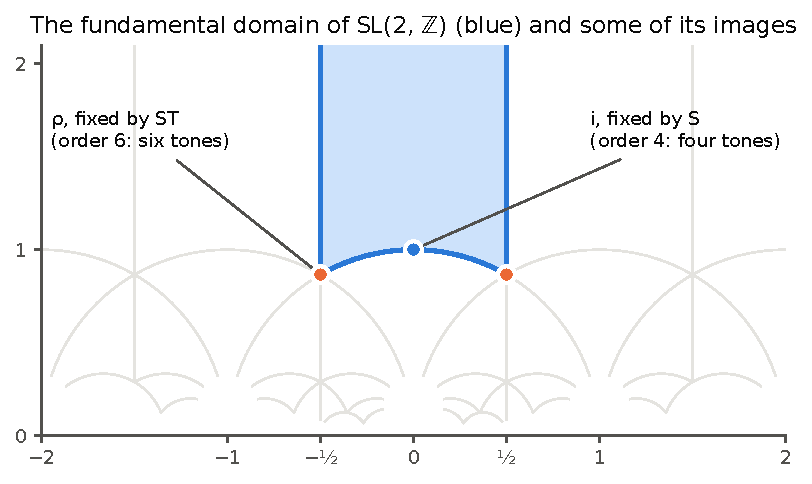
\includegraphics[width=0.82\textwidth]{tones-domain}
  \caption{The standard fundamental domain $\{|\mathrm{Re}\,\tau|\le\frac12,\ |\tau|\ge1\}$ of $\SL(2,\Z)$, some of its images, and the two elliptic points. Script: \script{twelve\_tones.py}.}
  \label{fig:domain}
\end{figure}

\section{The twelve characters}

A \emph{character} of $\SL(2,\Z)$ is a homomorphism to a commutative group.

\begin{theorem}\label{thm:char}
Let $\chi\colon \SL(2,\Z)\to A$ be a homomorphism to a commutative group.
Then $\chi(S) = \chi(T)^{-3}$ and $\chi(T)^{12} = 1$, and $\chi$ is determined by $\chi(T)$.
\end{theorem}

\begin{proof}
Apply $\chi$ to $S^2 = -1 = (ST)^3$.
Because $A$ is commutative, this gives $\chi(S)^2 = \chi(S)^3\chi(T)^3$, so $\chi(S)\chi(T)^3 = 1$.
Next, $S^4 = 1$ gives $1 = \chi(S)^4 = \chi(T)^{-12}$.
Finally, $S$ and $T$ generate the group, so $\chi(T)$ determines $\chi$.
\end{proof}

The Dedekind eta function $\eta(\tau) = e^{2\pi i\tau/24}\prod_{n\ge1}(1-e^{2\pi i n\tau})$ has two transformation laws.
The first, $\eta(\tau+1) = e^{2\pi i/24}\eta(\tau)$, follows from the product.
The second is the classical $\eta(-1/\tau)^2 = -i\tau\,\eta(\tau)^2$ \cite{Apostol}.
Write $(f|_1\gamma)(\tau) = (c\tau+d)^{-1}f(\gamma\tau)$ for the weight-one action.

\begin{theorem}\label{thm:eta}
There is a character $\chi_\eta\colon\SL(2,\Z)\to\C^\times$ with $\eta^2|_1\gamma = \chi_\eta(\gamma)\,\eta^2$ for every $\gamma$, and
\[
  \chi_\eta(T) = e^{2\pi i/12},\qquad \chi_\eta(S) = -i = e^{2\pi i\cdot 9/12}.
\]
Every character $\SL(2,\Z)\to\C^\times$ is one of the twelve distinct powers $\chi_\eta^k$, $0\le k<12$.
\end{theorem}

\begin{proof}
The set of $\gamma$ with $\eta^2|_1\gamma\in\C\,\eta^2$ is a subgroup, because $\eta^2$ has no zeros.
It contains $T$ and $S$ by the two transformation laws, so it is all of $\SL(2,\Z)$.
The scalar is unique and multiplicative.
For the last statement, let $\chi$ be any character.
Theorem~\ref{thm:char} gives $\chi(T)^{12} = 1$.
Since $e^{2\pi i/12}$ is a primitive 12th root of unity, $\chi(T) = \chi_\eta(T)^k$ for some $k < 12$.
Theorem~\ref{thm:char} then gives $\chi = \chi_\eta^k$.
\end{proof}

So the character group of $\SL(2,\Z)$ is cyclic of order~12, generated by the multiplier of $\Delta^{1/12}$, where $\Delta = \eta^{24}$ is Ramanujan's cusp form.
This is the dual form of the classical isomorphism $\SL(2,\Z)^{\mathrm{ab}}\cong\Z/12$.
Theorems~\ref{thm:char} and~\ref{thm:eta} are proved in Lean~4 with Mathlib in \formal{} (\texttt{tau-track/TauTrack/Tones}).
The law for $\eta(-1/\tau)^2$ is taken from the TauCeti library.
The script \script{twelve\_tones.py} also checks $\eta^2|_1\gamma = \chi_\eta(\gamma)\eta^2$ numerically, to 40 digits, for 200 random words in $S^{\pm1}$, $T^{\pm1}$.

\section{The pitch map}

Write $\chi_\eta(\gamma) = e^{2\pi i\,p(\gamma)/12}$ with $p(\gamma)\in\Z/12$.
Then $p\colon\SL(2,\Z)\to\Z/12$ is a surjective homomorphism.
We call $p(\gamma)$ the \emph{pitch} of $\gamma$, and read $\Z/12$ as the twelve pitch classes with $C = 0$.

\begin{center}
\begin{tabular}{@{}lll@{}}
\toprule
element & pitch & interval\\
\midrule
$T$ & 1 & semitone up\\
$S$ & 9 & minor third down\\
$ST$ & 10 & whole tone down\\
$(ST)^2$ & 8 & major third down\\
$-1 = S^2 = (ST)^3$ & 6 & tritone\\
\bottomrule
\end{tabular}
\end{center}

\noindent
The stabilisers of the elliptic points map onto the subgroups of order 4 and~6 (Figure~\ref{fig:clock}).
\begin{itemize}
\item The powers of $S$, which fix~$i$, have pitches $\{0,3,6,9\}$: the diminished-seventh chord C--E$\flat$--F$\sharp$--A.
\item The powers of $ST$, which fix~$\rho$, have pitches $\{0,2,4,6,8,10\}$: the whole-tone scale.
\item The powers of $(ST)^2$ have pitches $\{0,4,8\}$: the augmented triad.
\end{itemize}
These, with the tritone $\{0,6\}$, are the subgroups of $\Z/12$.
They are among the maximally even sets of music theory \cite{CloughDouthett}.

\begin{figure}[ht]
  \centering
  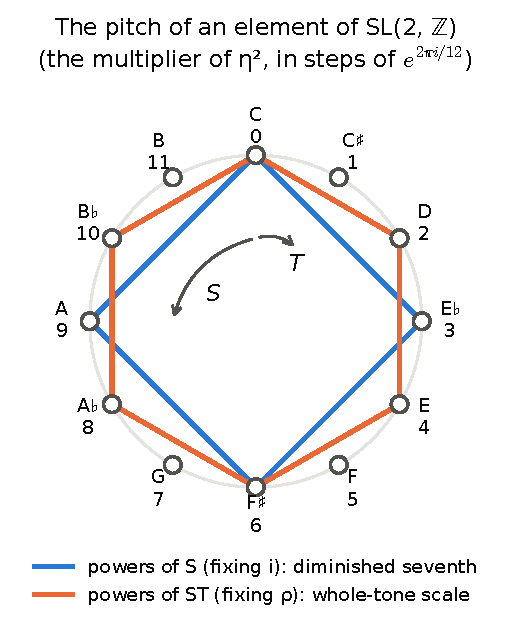
\includegraphics[width=0.5\textwidth]{tones-clock}
  \caption{The pitch map. The stabiliser of the Gaussian point $i$ sounds the diminished seventh; the stabiliser of the Eisenstein point $\rho$ sounds the whole-tone scale.}
  \label{fig:clock}
\end{figure}

\section{The circle of fifths is a Galois group}

The automorphisms of $\Z/12$ are multiplication by the units $\{1,5,7,11\}$.
Every unit squares to~1, so they form the Klein four-group.
In music theory they are known as the multiplicative operations.
$M_7$ sends the chromatic scale to the circle of fifths, $M_5$ to the circle of fourths, and $M_{11}$ is inversion.

The same group is $\Gal(\Q(\zeta_{12})/\Q)$, with $\sigma_a(\zeta_{12}) = \zeta_{12}^a$.
Its three subgroups of order two fix the three quadratic subfields of $\Q(\zeta_{12}) = \Q(i,\sqrt{-3})$:
\[
  \Q(i)\ \text{fixed by}\ \{1,5\},\qquad \Q(\sqrt{-3})\ \text{fixed by}\ \{1,7\},\qquad \Q(\sqrt3)\ \text{fixed by}\ \{1,11\}.
\]
So the circle of fifths $M_7$ is the automorphism that fixes the Eisenstein field and moves the Gaussian one.
Dually, the four Dirichlet characters modulo 12 are the trivial character and the characters of these fields:

\begin{center}
\begin{tabular}{@{}lrrrrl@{}}
\toprule
character & 1 & 5 & 7 & 11 & $L(1,\chi)$\\
\midrule
$\chi_{-4}$ & $1$ & $1$ & $-1$ & $-1$ & $\pi/4$\\
$\chi_{-3}$ & $1$ & $-1$ & $1$ & $-1$ & $\pi/(3\sqrt3)$\\
$\chi_{12} = \chi_{-4}\chi_{-3}$ & $1$ & $-1$ & $-1$ & $1$ & $\log(2+\sqrt3)/\sqrt3$\\
\bottomrule
\end{tabular}
\end{center}

\noindent
The values $L(1,\chi)$ are given by the class number formula \cite{Davenport}.
The script computes them from the digamma function and checks them to 35 digits.
The Dedekind zeta function of $\Q(\zeta_{12})$ factors as $\zeta(s)L(s,\chi_{-4})L(s,\chi_{-3})L(s,\chi_{12})$ \cite{Washington}.
So each of the four ``tones'' of the Klein group carries an $L$-function.

\section{The diatonic scale}

The diatonic scale $\{0,2,4,5,7,9,11\}$ has two classical descriptions.
\begin{itemize}
\item It is seven consecutive fifths (F, C, G, D, A, E, B).
\item It is maximally even: it is $\{\lfloor 12k/7\rfloor + 11 : 0\le k<7\}$ \cite{CloughDouthett}.
\end{itemize}
Its step pattern LLsLLLs is a rotation of the Christoffel word LLLsLLs of slope $2/5$, the Lydian mode.
The other rotations are the other six modes.
These finite statements are proved in Lean by computation and checked by the script.

\section{Why twelve? Two different reasons}

\paragraph{The modular reason.}
$\SL(2,\Z)$ is the amalgamated product $\Z/4 *_{\Z/2}\Z/6$ of the two stabilisers over their common centre $\{\pm1\}$ \cite{Trees}.
Its abelianisation therefore has order $4\cdot6/2 = 12$.
The same orders give its Euler characteristic $\frac14+\frac16-\frac12 = -\frac1{12}$, which equals $\zeta(-1)$.
This equality is a case of Harder's Gauss--Bonnet theorem \cite{Harder}.
The weight 12 of $\Delta$ has a related source: in the valence formula the two elliptic points contribute $\frac12$ and $\frac13$, and this is what makes 12 the smallest weight of a cusp form \cite{Serre}.

\paragraph{The acoustic reason.}
Equal temperament with $n$ steps approximates the fifth $3/2$ by $2^{k/n}$.
The best choices come from the continued fraction
\[
  \log_2\tfrac32 = [0;1,1,2,2,3,1,5,2,\dots],\qquad \text{convergents}\ \tfrac12,\ \tfrac35,\ \tfrac7{12},\ \tfrac{24}{41},\ \tfrac{31}{53},\dots
\]
The 12-step fifth is 1.955 cents flat.
No $n<29$ does better, and $n=41$ and $n=53$ do much better (Figure~\ref{fig:temp}).
Twelve wins because it is the smallest number of steps with a good fifth.

\begin{figure}[ht]
  \centering
  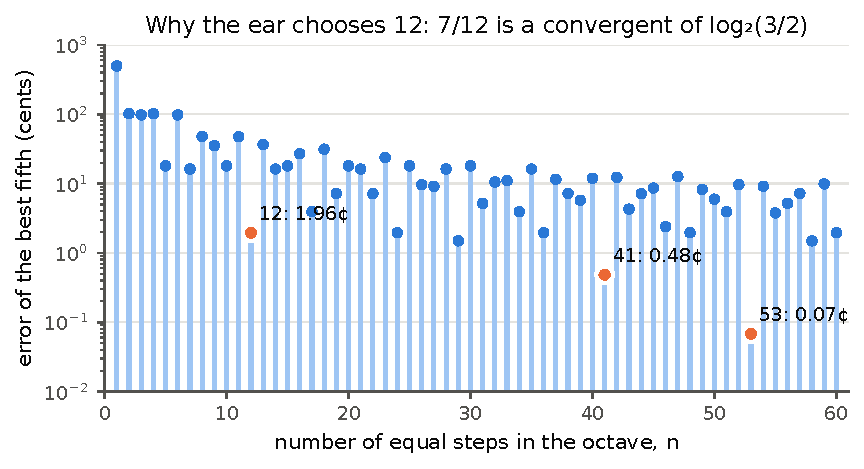
\includegraphics[width=0.82\textwidth]{tones-temperaments}
  \caption{Error of the best fifth in $n$-step equal temperament. The convergents 12, 41, 53 of $\log_2(3/2)$ stand out.}
  \label{fig:temp}
\end{figure}

\paragraph{What the dictionary does and does not show.}
The pitch map is exact.
The modular group's characters, the automorphisms of the chromatic circle and the quadratic subfields of $\Q(\zeta_{12})$ are one structure, $\Z/12$ with its Klein group of automorphisms.
The dictionary does not explain why musicians use twelve notes.
That comes from $\log_2(3/2)$, a quantity that does not appear in the modular reason.
The author's working hypothesis is that the two appearances of twelve are linked.

\begin{question}
Is there a mechanism, physical or perceptual, by which the arithmetic of $\SL(2,\Z)$ or of $\Q(\zeta_{12})$ constrains musical tuning or harmony?
For example, is the special role of the diminished seventh and the whole-tone scale (the elliptic stabilisers) visible in psychoacoustic data?
\end{question}

\section*{Status of the statements}

\begin{center}
\small
\begin{tabular}{@{}p{0.62\textwidth}l@{}}
\toprule
Statement & Grade\\
\midrule
Theorem~\ref{thm:char}; Theorem~\ref{thm:eta}; the pitch table; the stabiliser chords & \gradeLean{} and \gradeComputed\\
$(\Z/12)^\times$ is the Klein group; the fixed fields; fifths, maximal evenness & \gradeLean{} and \gradeComputed\\
$L(1,\chi)$ for the characters mod 12; Dedekind zeta factorisation & \gradeClassical{}, values \gradeComputed\\
Continued fraction of $\log_2(3/2)$ and the temperament errors & \gradeComputed\\
The two twelves are linked & \gradeOpen{} (working hypothesis)\\
\bottomrule
\end{tabular}
\end{center}

\noindent
\textsc{lean}: proved in Lean 4 with Mathlib.
\textsc{classical}: a published theorem.
\textsc{computed}: checked numerically by a script in this repository.
\textsc{open}: a question, not a result.

\begin{thebibliography}{9}
\bibitem{Apostol} T.~M. Apostol, \emph{Modular Functions and Dirichlet Series in Number Theory}, 2nd ed., Springer, 1990.
\bibitem{CloughDouthett} J.~Clough and J.~Douthett, Maximally even sets, \emph{J. Music Theory} 35 (1991), 93--173.
\bibitem{Davenport} H.~Davenport, \emph{Multiplicative Number Theory}, 3rd ed., Springer, 2000.
\bibitem{Harder} G.~Harder, A Gauss--Bonnet formula for discrete arithmetically defined groups, \emph{Ann. Sci. \'Ec. Norm. Sup.} 4 (1971), 409--455.
\bibitem{Serre} J.-P. Serre, \emph{A Course in Arithmetic}, Springer, 1973.
\bibitem{Trees} J.-P. Serre, \emph{Trees}, Springer, 1980.
\bibitem{Washington} L.~C. Washington, \emph{Introduction to Cyclotomic Fields}, 2nd ed., Springer, 1997.
\end{thebibliography}

\end{document}
